\documentclass{article}
\usepackage[left=3cm,right=3cm,top=2.5cm,bottom=2cm]{geometry} % page settings
\usepackage{amsmath} % provides many mathematical environments & tools
\usepackage{amssymb}
\usepackage{amsfonts}
\usepackage[spanish]{babel}
\usepackage[bookmarks]{hyperref}

\usepackage{multirow}

\usepackage{algorithm}
\usepackage{algpseudocode}
\usepackage{pifont}

\usepackage[utf8]{inputenc}
\setlength{\parindent}{0mm}

\usepackage[parfill]{parskip}

% Para el código
\usepackage{listings}
\usepackage{xcolor}
\definecolor{gray}{rgb}{0.5,0.5,0.5}
\newcommand{\n}[1]{{\color{gray}#1}}
\lstset{numbers=left,numberstyle=\small\color{gray}}

% Entorno para estilo de ejercicios
\setlength{\parindent}{0pt}

\usepackage{color}   %May be necessary if you want to color links
\usepackage{hyperref}
\hypersetup{
    colorlinks=true, %set true if you want colored links
    linktoc=all,     %set to all if you want both sections and subsections linked
    linkcolor=blue,  %choose some color if you want links to stand out
}

\usepackage{graphicx}
\usepackage{subfig}

\usepackage{listings,textcomp}
\title{Problema del viajante de comercio\\ Travelling salesman problem}
\author{José Antonio Álvarez Ocete - Norberto Fernández de la Higuera \\ Javier Gálvez Obispo - Yábir García Benchakhtir }
\date{\today}

% Custom
\providecommand{\abs}[1]{\lvert#1\rvert}
\setlength\parindent{0pt}
\definecolor{Light}{gray}{.90}
\newcommand\ddfrac[2]{\frac{\displaystyle #1}{\displaystyle #2}}

% Listings
\lstset{literate=   % listings config
  {á}{{\'a}}1 {é}{{\'e}}1 {í}{{\'i}}1 {ó}{{\'o}}1 {ú}{{\'u}}1
  {Á}{{\'A}}1 {É}{{\'E}}1 {Í}{{\'I}}1 {Ó}{{\'O}}1 {Ú}{{\'U}}1
  {à}{{\`a}}1 {è}{{\`e}}1 {ì}{{\`i}}1 {ò}{{\`o}}1 {ù}{{\`u}}1
  {À}{{\`A}}1 {È}{{\'E}}1 {Ì}{{\`I}}1 {Ò}{{\`O}}1 {Ù}{{\`U}}1
  {ä}{{\"a}}1 {ë}{{\"e}}1 {ï}{{\"i}}1 {ö}{{\"o}}1 {ü}{{\"u}}1
  {Ä}{{\"A}}1 {Ë}{{\"E}}1 {Ï}{{\"I}}1 {Ö}{{\"O}}1 {Ü}{{\"U}}1
  {â}{{\^a}}1 {ê}{{\^e}}1 {î}{{\^i}}1 {ô}{{\^o}}1 {û}{{\^u}}1
  {Â}{{\^A}}1 {Ê}{{\^E}}1 {Î}{{\^I}}1 {Ô}{{\^O}}1 {Û}{{\^U}}1
  {œ}{{\oe}}1 {Œ}{{\OE}}1 {æ}{{\ae}}1 {Æ}{{\AE}}1 {ß}{{\ss}}1
  {ű}{{\H{u}}}1 {Ű}{{\H{U}}}1 {ő}{{\H{o}}}1 {Ő}{{\H{O}}}1
  {ç}{{\c c}}1 {Ç}{{\c C}}1 {ø}{{\o}}1 {å}{{\r a}}1 {Å}{{\r A}}1
  {€}{{\EUR}}1 {£}{{\pounds}}1 {ñ}{{\~{n}}}1
}

\lstset{    %listings config
	language=C++,
	belowcaptionskip=1\baselineskip,
	breaklines=true,
	frame=L,
	xleftmargin=0.1in,
	%otherkeywords={},
	showstringspaces=false,
	backgroundcolor=\color{white},
	basicstyle=\footnotesize\ttfamily,
	keywordstyle=\bfseries\color{purple!90!black},
	commentstyle=\itshape\color{gray!85!},
	identifierstyle=\color{blue!80!black},
	stringstyle=\color{green!60!black},
}

\begin{document}

\maketitle
\newpage
\tableofcontents
\newpage

\section{Descripción del problema}

En el problema del viajante de comercio (\textit{Travelling Salesman
  Problem}) se nos dan las coordenadas de un conjunto finito de
ciudades y se nos pide encontrar un recorrido de las misma de forma
que la distancia que recorramos sea la menor posible.

\section{Soluciones greedy}

\subsection{Nearest Neighbor}

Teniendo como conjunto de ciudades $\Omega$ y la matriz $\mathcal{M}$ 
que contiene la distancia entre cada una de las ciudades, partimos de
$\mathcal{C}$  el conjunto de posibles candidatos (su valor inicial es
$\Omega$) y el conjunto solución $\mathcal{R}$ (se inicializa vacío).

Mediante ésta estructura el algoritmo se puede clasificar como greedy, 
teniendo en cuenta que a cada iteración del algoritmo se busca el óptimo 
local (la ciudad más cercana a la actual) y todos los candidatos usados 
pasan al conjunto solución $\mathcal{R}$, descartándolos del conjunto 
$\mathcal{C}$.


El funcionamiento del algoritmo sería el siguiente:

\begin{algorithm}[H]
\caption{Nearest Neighbor}
\begin{algorithmic}
\State $\mathcal{R}$ = [random()$\%|$ $\Omega$ $|$]
\State $\mathcal{C}$ - $\mathcal{R}$[0]
\For{pos in [0,n-2]}
\State bestPos = nearest($\mathcal{M}$[$\mathcal{R}$[pos]],$\mathcal{C}$)
\State $\mathcal{R}$.push($\mathcal{C}$[bestPos])
\State $\mathcal{C}$.erase(bestPos)
\EndFor
\State return $\mathcal{R}$
\end{algorithmic}
\end{algorithm}

Donde la función "nearest" devuelve la posición de la ciudad que, de entre 
todos los candidatos, está más cerca a la actual.

El algoritmo es O(n²) ya que tiene la misma estructura que el algoritmo de
ordenación por selección, donde se escogía el valor mínimo de las componentes 
que no se habían insertado todavía. En nuestro caso se escoge la ciudad que 
es la más cercana a la actual y se incluye en el conjunto solución, a partir 
del cual se repetirá el mismo procedimiento.

\subsection{Cheapest Insertion}

Si tomamos $\Omega$ el conjunto de ciudades, donde cada ciudad la
notamos como $\omega$ y $\mathcal{M}$ la matriz simetrica de la
distancia entre las ciudades.

Para este tomamos $<i,j>$ tales que $min(M) = M_{ij}$. Partimos de la
solución $\Gamma = \{ \omega_i, \omega_j \} $ y en cada iteración
buscamos la ciudad de índice $p$ tal que $\omega_p \notin \Gamma$ y que minimiza:

\[
  M_{ip} + M_{jp} - M_{ij}
\]

Una implementación en pseudo-codigo sería:

\begin{algorithm}[H]
\caption{Cheap Insert}
\begin{algorithmic}
\State i, j = nodes(min($M$))
\State path = [i, j]
\State $\mathcal{C}$ = $\Omega$ - path
\While{C not empty}
\For{city in cities}
\If{city not in path}
\For{node in path}
\State T = minimizeDistance(node, city, node+1)
\EndFor
\State insert(path, T)
\State remove($\mathcal{C}$, T)
\EndIf
\EndFor
\EndWhile
\State return path
\end{algorithmic}
\end{algorithm}

Este algoritmo es un algoritmo claramente greedy donde:

\begin{itemize}
\item Nuestro conjunto de candidatos es el conjunto $\Omega$.
\item Mantenemos una lista de candidatos ya usados.
\item Como criterio para determinar si $\Gamma$ es valido buscamos no
  tener ciclos y que no se repitan los nodos.
\item Nuestra función de selección es la definida en algoritmo
  anterior y que determina en cada situación cual es la menor
  distancia que podemos agregar.
\item La función que nos permite comparar soluciones es la distancia
  del camino final $\Gamma$
\end{itemize}

La eficiencia de este algoritmo es $(n^3)$ que no es de las mejores
pero nos aporta soluciones muy buenas como podremos ver en la parte
comparativa.

\subsection{Farthest insertion}

\begin{algorithm}[H]
\caption{Cheap Insert}
\begin{algorithmic}
\State i, j = nodes(max($M$))
\State path = [i, j]
\State $\mathcal{C}$ = $\Omega$ - path
\While{C not empty}
\For{city in cities}
\If{city not in path}
\For{node in path}
\State T = maximize(node, city, node+1)
\EndFor
\State insert(path, T)
\State remove($\mathcal{C}$, T)
\EndIf
\EndFor
\EndWhile
\State return path
\end{algorithmic}
\end{algorithm}

Este algoritmo es parecido al anterior pero en lugar de primar las
distancias más cortas buscamos aquellas que son mas largas. La
eficiencia es similar a la anterior.

\section{Otro algoritmo posible}

Finalmente hemos implementado una tercera estrategia basada en un
algoritmo genético. Dadas las dimensiones del problema (NP-completo),
es natural buscar una solución lo suficientemente buena aunque no
tenga por qué ser la mejor. Este es exactamente el punto de vista que
hemos tomado para abordar esta tercera solución.

Los algoritmos genéticos son un tipo de estrategias clasificadas como
metaheurísticas. Esto es, utilizadas en ámbitos muy diversos ya que
operan de forma abstracta e independiente al problema en si. En
particular, los algoritmos genéticos se basan en la teoría evolutiva
de Darwin en la que una población, mediante cruces entre sus
individuos y mutaciones, es cada vez más fuerte conformen pasan las
generaciones. Para más información sobre el tema:

\begin{verbatim}
https://es.wikipedia.org/wiki/Metaheuristica
http://sci2s.ugr.es/graduateCourses/Metaheuristicas
https://es.wikipedia.org/wiki/Algoritmo_geneticos
\end{verbatim}

En un algoritmo genético consideramos un conjunto o población de
soluciones (también llamados genes o individuos de la población),
inicializadas aleatoriamente, y realizamos distintas operaciones sobre
ellas para ir mejorándolas y así obtener soluciones cada vez
mejores. En nuestro caso, cada individuo será una permutación de
números: el orden en el que recorremos las ciudades.

Las operaciones que se realizan sobre los individuos son operadores de
cruce y operadores de mutación:
\begin{itemize}
\item Los operadores de cruce obtienen uno o varios individuos (hijos)
  a partir un par de soluciones de la poblacion (padres). En nuestro
  caso utilizaremos el operador de cruce de orden:
	
	\begin{figure}[H]
		\centering
		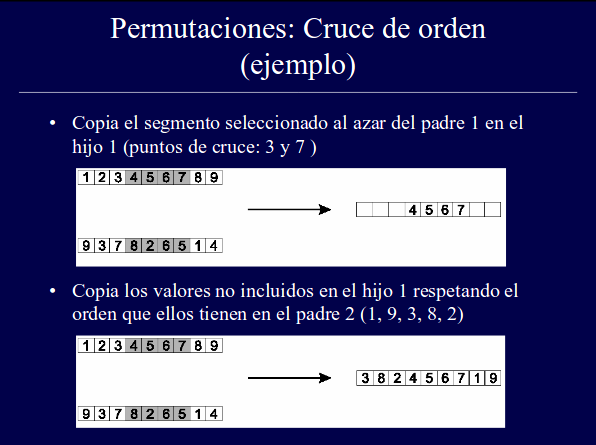
\includegraphics[width=0.8\textwidth]{imag1.png}
		\caption{Operador de cruce de orden.}
	\end{figure}
	
      \item Los operadores de mutación están limitados por una cierta
        probabilidad fijada. Es decir, no todos los individuos de una
        población mutan. Se aplican sobre un único individuo y lo
        alteran unicamente a él. En nuestro caso utilizaremos el
        operador de mutación por inserción:
	
	\begin{figure}[H]
		\centering
		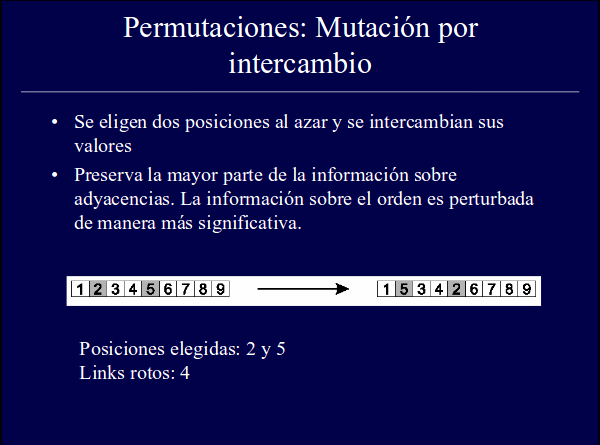
\includegraphics[width=0.8\textwidth]{imag2.png}
		\caption{Operador de mutación por intercambio.}
	\end{figure}
	
\end{itemize}
 
Ambos imágenes provienendel siguiente enlace, diapositivas 20 y 17 respectivamente:
http://users.exa.unicen.edu.ar/~icompevol/filminasenpdf/terceraclase.pdf

Además, hemos de medir cuan buena es cada una de nuestras soluciones,
necesitamos una \textbf{función de evaluación}. Esta será la longitud
de la ruta determinada por la permutación.

Finalmente y antes de explicar el flujo del algoritmo en si hace falta
definir un último operador: el de selección. Este operador define como
se realiza la selección de padres de una generación (si cogiesemos
unicamente los mejores convergeriamos muy rápido a un óptimo local
pues no hay diversidad en nuestra población mientras que si se
selecciona de forma puramente aleatoria nos estaríamos teniendo en
cuenta cuan buena es cada solución). Aplicaremos \textbf{selección por
  torneo}. En esta estrategia se seleccionan de forma aleatoria un
número pequeño de individuos (3 o 5 son valores comunmente
utilizados), y de entre estos se escoge el mejor.

Una vez definidos los operadores, el algoritmo en si es
sencillo. Realizaremos $n_generaciones$ generaciones a partir de una
poblacion de $N$ individuos obtenida aleatoriamente. En cada
generación se escogen padres (con el operador de selección) y se
cruzan (con el operador de cruce) hasta obtener una nueva generación
de $N$ elementos. Estos nuevos individuos se mutan (bajo una
probabilidad $mutate_probability$) y finalmente se sustituye la
población anterior por la nueva.

\begin{lstlisting}
InitializePopulation(population, pob_size, n_cities);
best_gen_ever = *population[0];
EvaluatePopulation(population, best_gen_ever, cities);

for (int i=0; i<n_generations; i++) {
	// Obtain the next generation and apply crossover from the elements of population
	ApplySelectionAndCrossover(population, new_generation);
	
	// Apply mutation to the new population with a probability prob
	ApplyMutation(new_generation, mutate_propability);
	
	// Evaluate the new population and save the best solution found
	EvaluatePopulation(new_generation, best_gen_ever, cities);
	
	// Replace the old population with the new one
	ReplaceGeneration(population, new_generation);
}
\end{lstlisting}

Nuestra mejor solución está almacenada en $best_gen_ever$.

\section{Conclusiones}

Como criterio para realizar las comparaciones entre algoritmos hemos usado la
distancia del recorrido obtenido como solución.

Se ha procedido a ejecutar todos los algoritmos con todos los mapas
usando el ordenador de Javier Galvez que cuenta con un i5-6200U con 4
núcleos a 2.3GHz, 8GB de RAM y ubuntu 16 LTS de 64 bits como sistema
operativo.

La siguiente gráfica recopila los resultados obtenidos:

\begin{figure}[H]
  \centering
  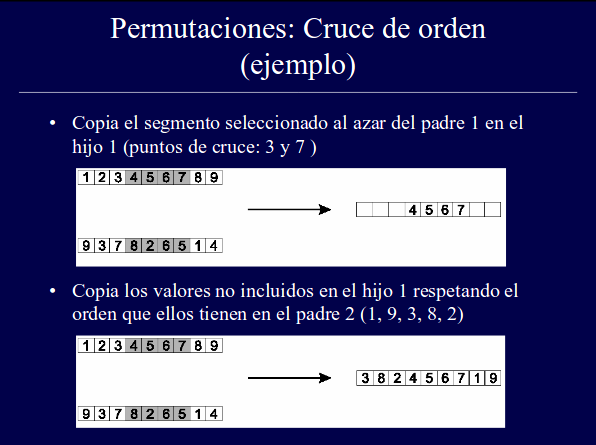
\includegraphics[width=0.8\textwidth]{imag1.png}
  \caption{Comparativa de distancias obtenidas.}
\end{figure}

Como se puede observar el algoritmo que ha logrado una mayor
eficiencia ha sido el algoritmo de \textit{Cheapest inserction}. Los
otros dos algoritmos greedy obtienen resultados parecidos en cuanto a
las distancias.

Claramente en este problema las soluciones propuestas vencen a la
solución propuesta como algoritmo genético.

Si consideramos importantes los tiempos de ejecución tenemos que
apreciar que el del vecino más cercanos obtiene tiempos más pequeños
debido a que su complejidad es solo $O(n^2)$ comparado con $O(n^3)$ de
los otros.

\end{document}